\subsection{Transformator}
I flyback converteren fungerer transformatoren lidt anderledes, i forhold til mange andre konstruktioner. Normalt vil der løbe en strøm i både den primære og sekundære vikling på samme tid. På den måde kan energien i transformatoren, transformeres direkte fra den primære vikling til den sekundære vikling. Det er ikke muligt i denne converter typologi, da der kun vil løbe strøm i én vikling ad gangen. Den energi, der skabes i den primære vikling, skal derfor kunne opbevares, indtil der begynder at løbe en strøm i sekundærviklingen. Sker det ikke, går kernen i mætning. Det vil sige, at der ikke er en lineær sammenhæng imellem transformatorens H- og B-felt.
Det sikres ved, at indsætte et luftgab i kernen, som øger den magnetiske modstand. Det gør, at kernen kan opbevare en større mængde energi.

I 1. iteration blev det valgt at tage udgangspunkt i en 1:1 transformator. Desuden er det i 2. iteration vigtigst, at få en velfungerende transformator. Derefter kan der senere optimeres på et mere optimalt viklingsforhold, hvis det vurderes nødvendigt. 

Med den estimerede nødvendige induktans beregnet i 1. iteration til $69.43\micro H$, blev energien, der induceres i primærviklingen udregnet til \begin{equation} \label{Primary_energy}
E = \frac{1} {2} \cdot L \cdot {I_{pk}}^2 = 0.996\milli J
\end{equation}

Energien skal kunne opbevares i kernen, for at undgå den føromtalte mætning. Hvornår en specifik transformator går i mætning, afhænger af selve kernen og dets materiale. Her faldt valget på en RM8 kerne og materialet 3f3, hvilket der er argumenteret for i sektion~\ref{Transana}.
På baggrund af databladet for 3f3, blev luftgabet designet efter at have et maksimalt B felt på $250mT$. Det gav et nødvendigt luftgap på:
\begin{equation} \label{Airgap}
l_g = \frac{L \cdot {I_{pk}}^2 \cdot \micro_0}{B^2 \cdot A_0} = 635.6\micro m
\end{equation}

Det gav en fornyet induktans på $53.31\micro H$. Herefter bruges $A_L$ for 3f3 materialet og induktansen til, at beregne vindingstallet, som blev udregnet og afrundet til 18 vindinger.
Analysen er herefter holdt op imod simuleringen i p-spice, for at sikre analyse og simulering stemmer overens.
 
Viklingen af transformatoren er sket med en kobbertråd, med en diameter på $0.425mm$. Det er en tyndere tråd end analyseret. Det kommer af, at der med den forventede trådtykkelse på $0.45mm$, ikke i praksis kunne vikles 18 vindinger. Det har samtidig øget vindingstallet til 19, for stadig at udnytte kernens bredde bedst muligt. Igen for at fylde kernen ud, er der for både primær- og sekundærsiden viklet 3 viklinger i parallel, for at udnytte højden af kernen. Det giver samlet den tredobbelte højde med 6 viklinger i alt, hvilet ender på $2.55mm$. Viklingen er udført ved skiftevis, at vikle en primærvikling og en sekundærvikling. På den måde optimeres koblingen i transformatoren. Imellem viklingerne indsættes tape, for at sikre det holdes fast. På figur~\ref{fig: viklingsoverblik} vises et overblik over viklingerne og dimensionerne. 
\begin{figure}[H]
	\center
	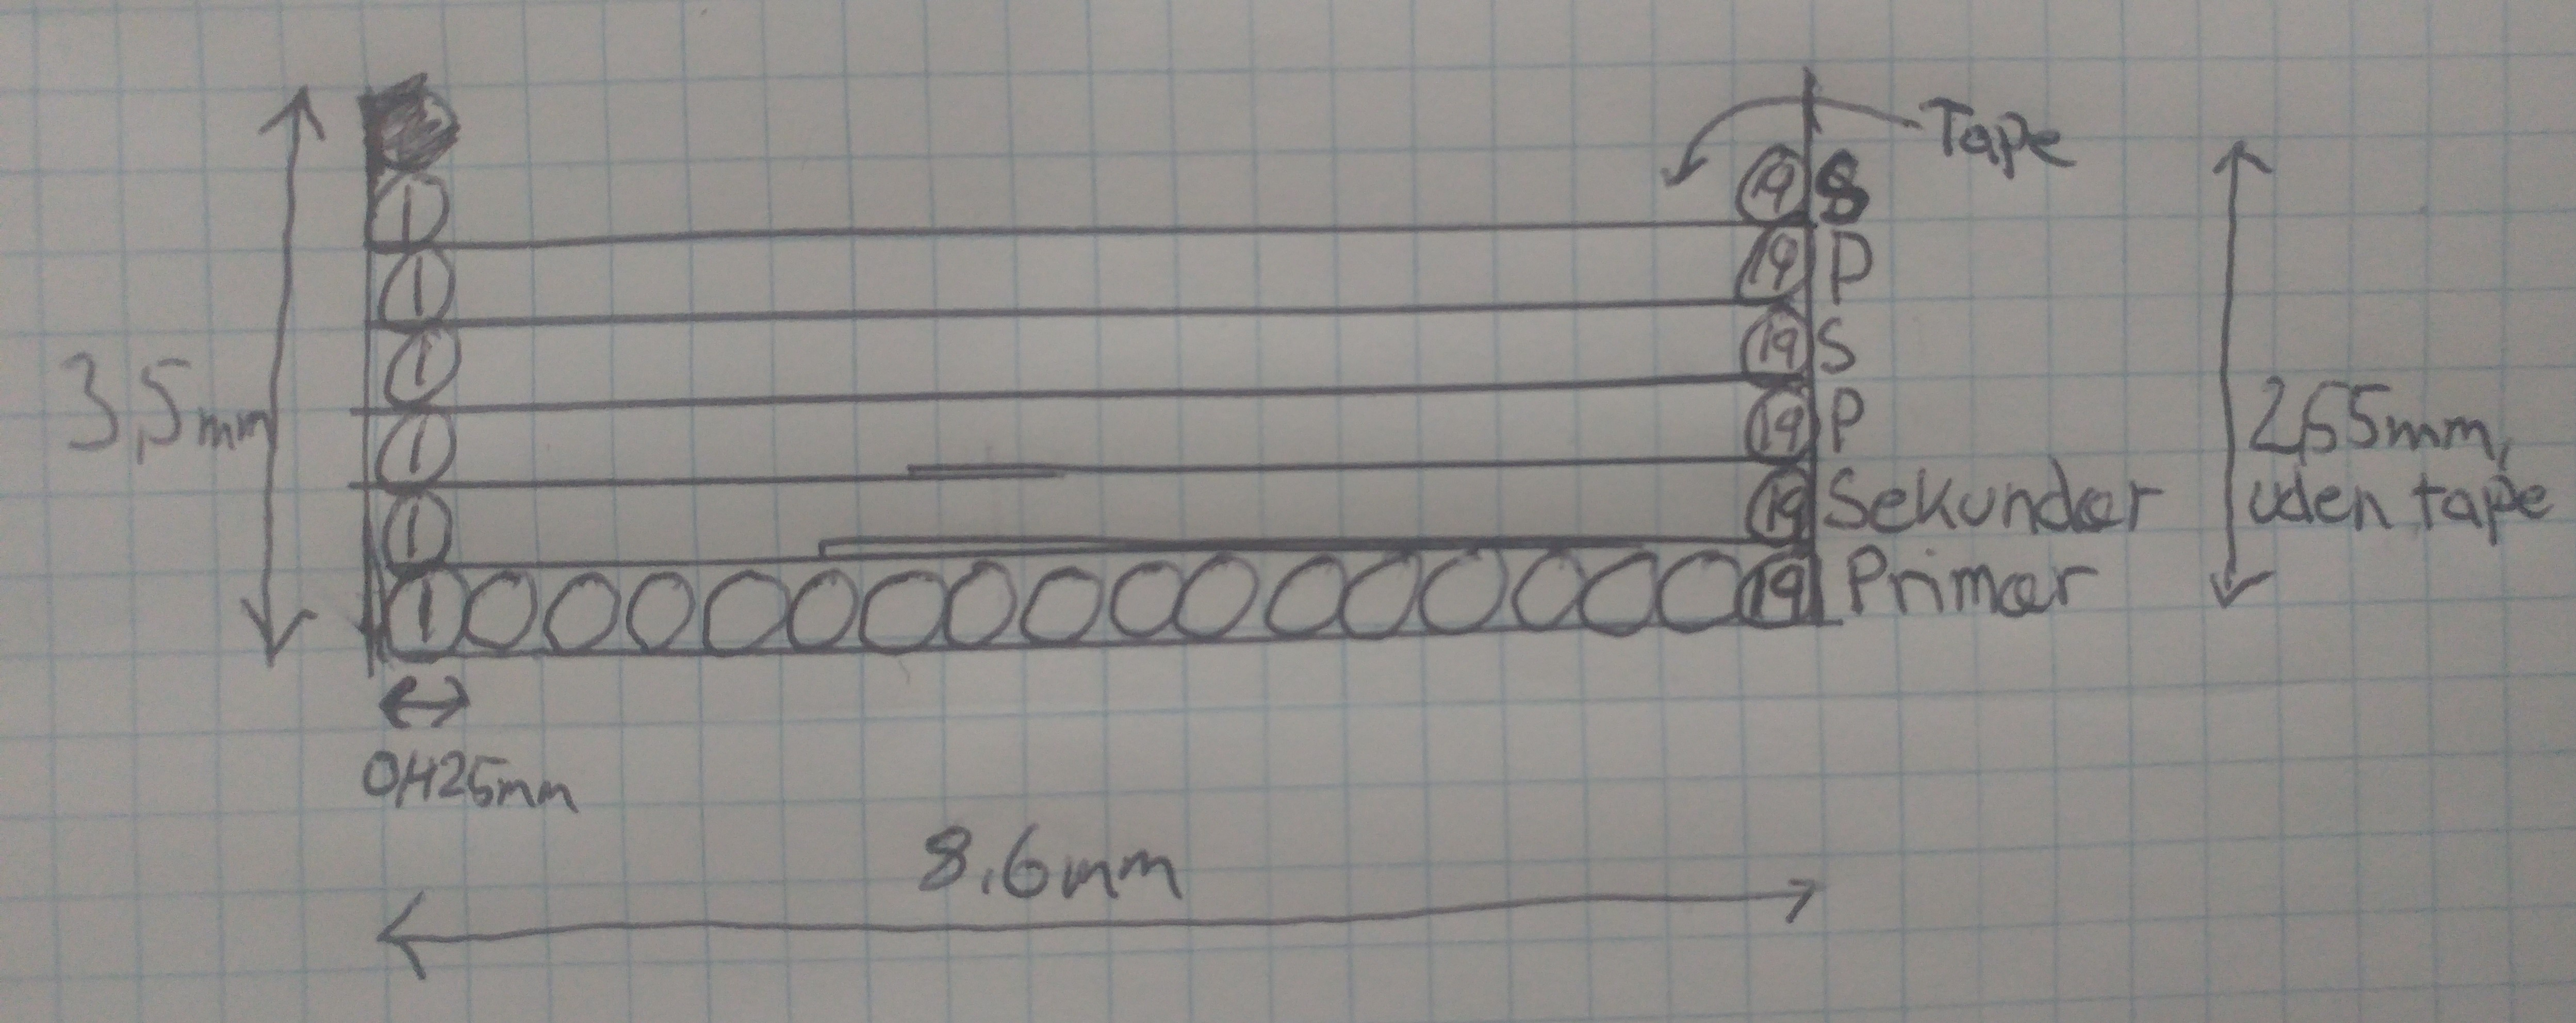
\includegraphics[max width=0.7\linewidth]{/tex/implementering/2iteration/billeder/transformatortegning.jpg}
	\caption{Overblik over viklingsantal og tykkelse}
	\label{fig: viklingsoverblik}
\end{figure}
\noindent Med vindingstallet på 19 istedet for 18, er selvinduktionen og dermed strømmene i transformatoren igen korrigeret. Herunder ses den endelig analyserede selvinduktion, ripplestrøm og peakstrøm for den viklede transformator.
\begin{equation} \label{L_2}
L_2 = N^2 \cdot A_L = 57.76\micro H
\end{equation}
\begin{equation} \label{I_ripple_final}
I_{ripple} = \frac{V_{inmin} \cdot D_{max}}{L_2 \cdot f_s} = 2.01A
\end{equation}
\begin{equation} \label{I_pk_final}
I_{pk} = \frac{V_{out} \cdot I_{out}}{V_{inmin} \cdot D_{maks}} + \frac{I_{ripple}}{2} = 5.53A
\end{equation}
Den implementerede transformator ses på figur~\ref{fig: Viklettrans}
\begin{figure}[H]
	\center
	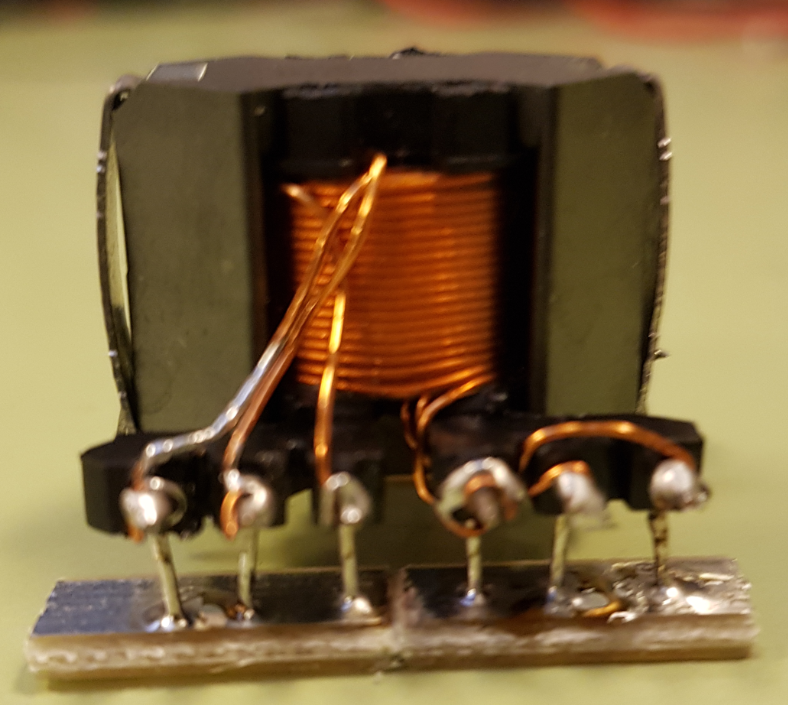
\includegraphics[max width=0.5\linewidth]{../dokumentation/tex/2iteration/billeder/Viklet_transformator.PNG}
	\caption{Viklet transformator}
	\label{fig: Viklettrans}
\end{figure}
\noindent Testen af transformatoren er udført ved, at måle selvinduktionen i primær- og sekundærviklingerne samt spredningsselvinduktionen. Det er gjort med en impedansmåler. Her er der benyttet så korte ledninger som muligt samt 4-wire teknikken, for at undgå ekstra induktans fra ledningerne. 

Selvinduktionen i primærviklingen måles henover primærviklingens to sider, mens sekundærviklingen holdes åben. Her laves et frekvenssweep fra $100Hz$ til $1MHz$. Samme fremgangsmåde for sekundærvikligen kan benyttes, men da transformatoren er 1:1, bør det være det samme.
Spredningsselvinduktionen måles samme sted, henover primærviklingen, hvor sekundærviklingen er kortsluttet. En ideel transformator vil give 0 i sådan en måling. Det betyder, at induktansen målt her, svarer til spredningsselvinduktionen. 

For yderligere forklaring af design, implementering og test af transformatoren henvises til dokumentationen afsnit 5.1, hvor dette er uddybet.